\documentclass[a4paper]{article}

\usepackage[utf8]{inputenc}
\usepackage[T1]{fontenc}
\usepackage{textcomp}
\usepackage{amsmath, amssymb}
\usepackage{array,multirow,graphicx}
\usepackage{booktabs}
\usepackage{hyperref}
\usepackage{subcaption}
\usepackage{biblatex}
\addbibresource{report.bib}


% figure support
\usepackage{import}
\usepackage{xifthen}
\pdfminorversion=7
\usepackage{pdfpages}
\usepackage{transparent}
\newcommand{\incfig}[1]{%
	\def\svgwidth{\columnwidth}
	\import{./figures/}{#1.pdf_tex}
}

\pdfsuppresswarningpagegroup=1


\title{NPFL103 Information Retrieval: Assignment 2}
\date{\today}
\author{Andrew McIsaac}

\begin{document}
\maketitle

\section{Introduction}
This report explores using publicly available information retrieval frameworks
for retrieval on documents in both English and Czech. I use Elasticsearch, a
distributed, RESTful search engine. It is built on Apache Lucene, a Java library
which provides both indexing and search features. I explore and evaluate the
capabilities of Elasticsearch in terms of text analysis features, similarity
score weightings and measurements, and boosting of query terms.

\section{Preprocessing and Index Construction}

\section{Query Processing and Retrieval}

\section{Baseline Results}
With the constrained baseline results as specified in the assignment brief, my
system achieved a mean average precision (MAP) score of 0.0597 on the Czech
training topics, and a P$_{10}$ score of 0.0840. The averaged 11-point
precision/recall graph is shown in Fig. \ref{fig:cs_train}.

For the English documents, the baseline MAP score was 0.0445, with a P$_{10}$
score of 0.0840. The averaged 11-point precision/recall graph is shown in Fig.
\ref{fig:en_train}.

\begin{figure}[htpb]
	\centering
	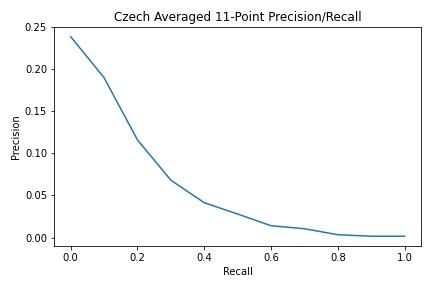
\includegraphics[width=0.8\textwidth]{plot_run-0_cs_precision_recall.jpg}
	\caption{Averaged 11-point Precision/Recall for Czech training data on run-0}
	\label{fig:cs_train}
\end{figure}

\begin{figure}[htpb]
	\centering
	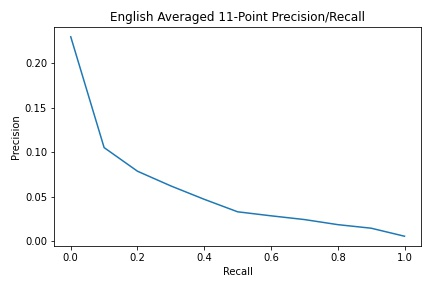
\includegraphics[width=0.8\textwidth]{plot_run-0_en_precision_recall.jpg}
	\caption{Averaged 11-point Precision/Recall for English training data on run-0}
	\label{fig:en_train}
\end{figure}

\section{Experiments}

\subsection{Preprocessing Methods for Indexing}
\label{sec:preproc}
I experimented with stopwords, lemmatization and stemming. In every case, I also
converted all words to lower case. The results are shown in Table
\ref{tab:terms}. 

\begin{table}[htpb]
	\centering
	\caption{Mean average precision (MAP) and $P_{10}$ precision of the first 10
		documents training performance with different preprocessing techniques.\\
	wf: word forms, sw: stopwords, l: lemmatization, s: stemming\\}
	\label{tab:terms}
	\begin{tabular}{@{}l|ccccc@{}}
		\toprule
		Language & & wf & sw & sw+l & sw+s \\
		\cmidrule(r){1-1}\cmidrule(lr){2-2}\cmidrule(lr){3-3}\cmidrule(lr){4-4}\cmidrule(lr){5-5}\cmidrule(l){6-6}
		English & MAP & 0.0445 & 0.1244 & 0.0834 & \textbf{0.1751} \\
				& \small{$P_{10}$} & \small{0.084} & \small{0.172} & \small{0.136} & \small{0.252} \\
		\cmidrule(r){1-1}\cmidrule(lr){2-2}\cmidrule(lr){3-3}\cmidrule(lr){4-4}\cmidrule(lr){5-5}\cmidrule(l){6-6}
		Czech & MAP & 0.0597 & 0.0770 & \textbf{0.1553} & 0.0672 \\
			  & \small{$P_{10}$} & \small{0.084} & \small{0.100} & \small{0.148} & \small{0.060} \\
		\bottomrule
	\end{tabular}
\end{table}

For English documents, preprocessing with stopwords lists and stemming produced
the best results, both for MAP and $P_{10}$, while using stopwords lists and
lemmas produced the best results for Czech documents.

\subsection{Term/Document Frequency Weighting}
I experimented with different term frequency and document frequency weighting
scores. From Table \ref{tab:tfidf} it can be seen that for both languages there
is significant performance improvement on the training data with natural term
frequency weighting, and either inverse document frequency or probabilistic idf
for both English and Czech documents, with prob idf marginally better than 
standard idf in both cases. Using a different term weighting than just term
frequency (logarithm or augmented) produced significantly weaker results.

\begin{table}[htpb]
	\centering
	\caption{Mean average precision (MAP) and $P_{10}$ precision of the first
		10 documents training performance with different tf-idf weightings.\\
	SMART notation tags are applied to both query and document in all cases.\\}
	\label{tab:tfidf}
	\begin{tabular}{@{}l|cccccc@{}}
		\toprule
		Language & & nnc & ntc & npc & ltc & apc \\
		\cmidrule(r){1-1}\cmidrule(lr){2-2}\cmidrule(lr){3-3}\cmidrule(lr){4-4}\cmidrule(lr){5-5}\cmidrule(lr){6-6}\cmidrule(l){7-7}
		English & MAP & 0.1751 & 0.2244 & \textbf{0.2248} & 0.1320 & 0.0469 \\
				& \small{$P_{10}$} & \small{0.252} & \small{0.328} & \small{0.328} & \small{0.172} & \small{0.092} \\
		\cmidrule(r){1-1}\cmidrule(lr){2-2}\cmidrule(lr){3-3}\cmidrule(lr){4-4}\cmidrule(lr){5-5}\cmidrule(lr){6-6}\cmidrule(l){7-7}
		Czech & MAP & 0.1553 & 0.1933 & \textbf{0.1947} & 0.0879 & 0.0922 \\
		& \small{$P_{10}$} & \small{0.148} & \small{0.224} & \small{0.228} & \small{0.096} & \small{0.100} \\
		\bottomrule
	\end{tabular}
\end{table}

\section{Run-1 Results}
b, k1 results for czech. Best map is 0.3, 0.6, 0.3362, p_10 0.348
{0.3: {0.6: 0.336187716348948, 0.8: 0.33570702166639926, 1: 0.3349692253899824, 1.2: 0.33101156577084007, 1.4: 0.32976067536004694, 1.6: 0.33295731817879465, 1.8: 0.33041062112064823, 2: 0.3283810038440958}, 0.4: {0.6: 0.3322993754803942, 0.8: 0.33228045453867544, 1: 0.33161805392496985, 1.2: 0.3277976465669487, 1.4: 0.32881373032947037, 1.6: 0.3273586006524154, 1.8: 0.3243283560839606, 2: 0.3218234945111043}, 0.5: {0.6: 0.33088985135306875, 0.8: 0.33238047500636336, 1: 0.3326451690182117, 1.2: 0.3286445140267687, 1.4: 0.329611920890378, 1.6: 0.3241983337266878, 1.8: 0.32040221954446646, 2: 0.3180449323954407}, 0.6: {0.6: 0.3293994496946114, 0.8: 0.3299325379288723, 1: 0.32682931545685406, 1.2: 0.3288139120563689, 1.4: 0.325831810962165, 1.6: 0.32208456989648626, 1.8: 0.31873107197778067, 2: 0.3154502383465029}, 0.65: {0.6: 0.32289647722335685, 0.8: 0.32324919117628476, 1: 0.32081035626196774, 1.2: 0.3250732105927023, 1.4: 0.3211360216781483, 1.6: 0.3170664316574522, 1.8: 0.31307108556639696, 2: 0.3109755154874409}, 0.7: {0.6: 0.31898696657180486, 0.8: 0.3176064828177939, 1: 0.31991081970174984, 1.2: 0.3180994134286236, 1.4: 0.31350826764917644, 1.6: 0.309472716876115, 1.8: 0.3082034565219011, 2: 0.30518736026223775}, 0.75: {0.6: 0.32016941419028266, 0.8: 0.31543354651160077, 1: 0.3181842479860423, 1.2: 0.3154561716392224, 1.4: 0.3116166451094655, 1.6: 0.30589876258053034, 1.8: 0.3017244883408625, 2: 0.29714344671419596}, 0.8: {0.6: 0.312578258979565, 0.8: 0.3095523559379068, 1: 0.31122668803480463, 1.2: 0.3117610959997985, 1.4: 0.30752215826378804, 1.6: 0.30181715581892704, 1.8: 0.294970584849406, 2: 0.2919406034574976}, 0.85: {0.6: 0.3089342023387328, 0.8: 0.30689486003673, 1: 0.3078847804738315, 1.2: 0.30237091151842377, 1.4: 0.29827068218904496, 1.6: 0.29328417460075007, 1.8: 0.28812958200662453, 2: 0.28460882348716776}, 0.9: {0.6: 0.3034114768737226, 0.8: 0.30024579132775614, 1: 0.3006151407812666, 1.2: 0.29698273430394484, 1.4: 0.2931168122429116, 1.6: 0.28595677706693295, 1.8: 0.2818331730674446, 2: 0.2769972833149585}, 0.95: {0.6: 0.2981116845281886, 0.8: 0.29922987120390937, 1: 0.2949887520066982, 1.2: 0.28879393796795205, 1.4: 0.28417040980610875, 1.6: 0.2773998320521102, 1.8: 0.27071314706701105, 2: 0.2654255176033051}}


b, k1 results for english. Best map is 0.5, 1.8, 0.345298, p_10 0.428
{0.3: {0.6: 0.32325565942397894, 0.8: 0.32827089949026195, 1: 0.3266131009667283, 1.2: 0.3319242286745161, 1.4: 0.33538921331057703, 1.6: 0.33794116086273623, 1.8: 0.33723507500911465, 2: 0.3347131080718353}, 0.4: {0.6: 0.32067306524896294, 0.8: 0.32230793551899756, 1: 0.33361352830110313, 1.2: 0.33879773698415616, 1.4: 0.3424889525905377, 1.6: 0.3451035999481531, 1.8: 0.3444048017989079, 2: 0.34074877470774}, 0.5: {0.6: 0.3217414171781537, 0.8: 0.32190306265706575, 1: 0.3311149978298885, 1.2: 0.33997642118507376, 1.4: 0.34002268930016155, 1.6: 0.3421469876471594, 1.8: 0.34529764126266616, 2: 0.3429105797859224}, 0.6: {0.6: 0.3175478438809756, 0.8: 0.32387011881519, 1: 0.3281577778360707, 1.2: 0.33841677951523086, 1.4: 0.3378416825035777, 1.6: 0.3396202322713936, 1.8: 0.340689553008865, 2: 0.33984435015780545}, 0.65: {0.6: 0.31729567449070173, 0.8: 0.3236373407617846, 1: 0.3296068312556232, 1.2: 0.33501824178827155, 1.4: 0.3383378706523042, 1.6: 0.33843696797503037, 1.8: 0.3387419744653402, 2: 0.3404768496986002}, 0.7: {0.6: 0.31712088031228863, 0.8: 0.32184947787456436, 1: 0.3293222986319796, 1.2: 0.3345080524892725, 1.4: 0.3380693685623598, 1.6: 0.3355560259886643, 1.8: 0.3382235571613383, 2: 0.33868240224889584}, 0.75: {0.6: 0.31746849974019664, 0.8: 0.3220919015298923, 1: 0.3296784537096358, 1.2: 0.33201451518739483, 1.4: 0.33573693768522384, 1.6: 0.33455105432562454, 1.8: 0.3350768485092363, 2: 0.33667566403942095}, 0.8: {0.6: 0.3176678757103372, 0.8: 0.3222204254185994, 1: 0.3308885687212964, 1.2: 0.3308335215405996, 1.4: 0.3306110594073923, 1.6: 0.3292568374454467, 1.8: 0.33040650106126895, 2: 0.32917840338316323}, 0.85: {0.6: 0.3176813834378884, 0.8: 0.3209832131546289, 1: 0.3288639171963772, 1.2: 0.326896059006214, 1.4: 0.33240550201540375, 1.6: 0.3324789854980645, 1.8: 0.3291260249705502, 2: 0.32736341813179104}, 0.9: {0.6: 0.31667601325681216, 0.8: 0.3230603546790172, 1: 0.3252394953138951, 1.2: 0.32447624281822973, 1.4: 0.32740754380546183, 1.6: 0.3297355079826818, 1.8: 0.3275548397863625, 2: 0.3248526116559649}, 0.95: {0.6: 0.31845662313774153, 0.8: 0.32115791769402446, 1: 0.32724261955286055, 1.2: 0.32447428169035797, 1.4: 0.32380418745397854, 1.6: 0.32268398674241267, 1.8: 0.3182885852790228, 2: 0.3161387051232342}}

lmjelinekmercer english 0.317428 czech 
lmdirichlet english 0.3232 czech 
dfr english 0.2957 czech 
dfi english 0.274287 czech 
ib english 0.343936 czech 

query boost 3 english 0.3332, p_10 0.392, czech 0.3405, p_10 0.3400
query boost 2 english 0.3339, p_10 0.388, czech 0.3409, p_10 0.3400
query boost 1 english 0.3367, p_10 0.396, czech 0.3420, p_10 0.3400
query boost 0.5 english 0.3444, p_10 0.4080, czech 0.3443, p_10 0.3440

fuzziness english , , czech 0.2426, 0.2680

best czech query phrase with 0.5 boost, bm25 0.3, 0.6, standard analyzer
best english bm25 0.3, 0.6, standard analyzer

\begin{figure}[htpb]
	\centering
	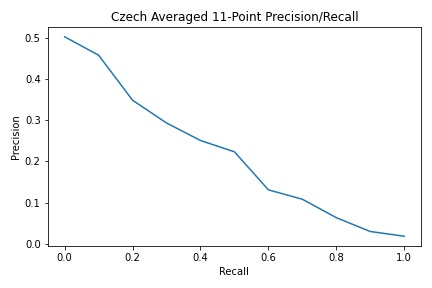
\includegraphics[width=0.8\textwidth]{plot_run-1_cs_precision_recall.jpg}
	\caption{Averaged 11-point Precision/Recall for Czech training data on run-1}
	\label{fig:cs_train_run_1}
\end{figure}

\begin{figure}[htpb]
	\centering
	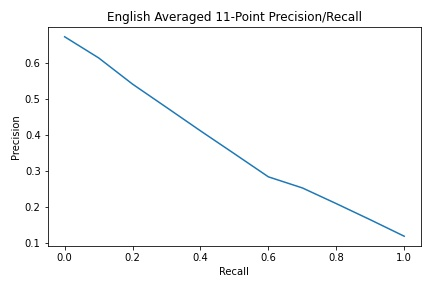
\includegraphics[width=0.8\textwidth]{plot_run-1_en_precision_recall.jpg}
	\caption{Averaged 11-point Precision/Recall for English training data on run-1}
	\label{fig:en_train_run_1}
\end{figure}

\section{Conclusion}

\printbibliography

\newpage

\appendix

\section{Set Up and Running Experiments}

Make sure all requirements are installed:
\begin{verbatim}
pip install -r requirements.txt
python -c "import spacy_udpipe; spacy_udpipe.download('cs')"
python -m spacy download en_core_web_sm
\end{verbatim}

To run experiments run the following commands, replacing \texttt{train} with
\texttt{test} where appropriate to obtain results for the test topics.
The program must be run from the parent directory of the documents.
\begin{verbatim}
python run.py -q topics-train_en.xml -d documents_en.lst -r run-0_en
    -o run-0_train_en.res

python run.py -q topics-train_cs.xml -d documents_cs.lst -r run-0_cs
    -o run-0_train_cs.res

python run.py -q topics-train_en.xml -d documents_en.lst -r run-1_en 
    -o run-1_train_en.res --stopwords --lowercase --stemming
    --df-weighting prob_idf --pivoted 0.85

python run.py -q topics-train_cs.xml -d documents_cs.lst -r run-1_cs
    -o run-1_train_cs.res --stopwords --lowercase --lemmas
    --df-weighting prob_idf --pivoted 0.9
\end{verbatim}

The program will create an inverted index or load a saved one based on the value
of the -r parameter.  That is, if the same run parameter has been called before,
there will be a saved index which does not need to be recreated, and the queries
can be run directly on that. Otherwise, it will construct a new one before
running the queries.

\end{document}
